\documentclass[_00_dissertation.tex]{subfiles}
\begin{document}

\onlyinsubfile{
    \renewcommand{\contentsname}{ОГЛАВЛЕНИЕ}
    \setcounter{tocdepth}{3}
    \tableofcontents
}

\refstepcounter{chapter}
\chapter*{\hfill ПРИЛОЖЕНИЕ~А}
\addcontentsline{toc}{chapter}{ПРИЛОЖЕНИЕ А Документы, подтверждающие практическое применение результатов диссертации}
\section*{Документы, подтверждающие практическое применение результатов диссертации}\label{section:Appendix_counterexample}

\begin{figure}[ht!]
    \centering
    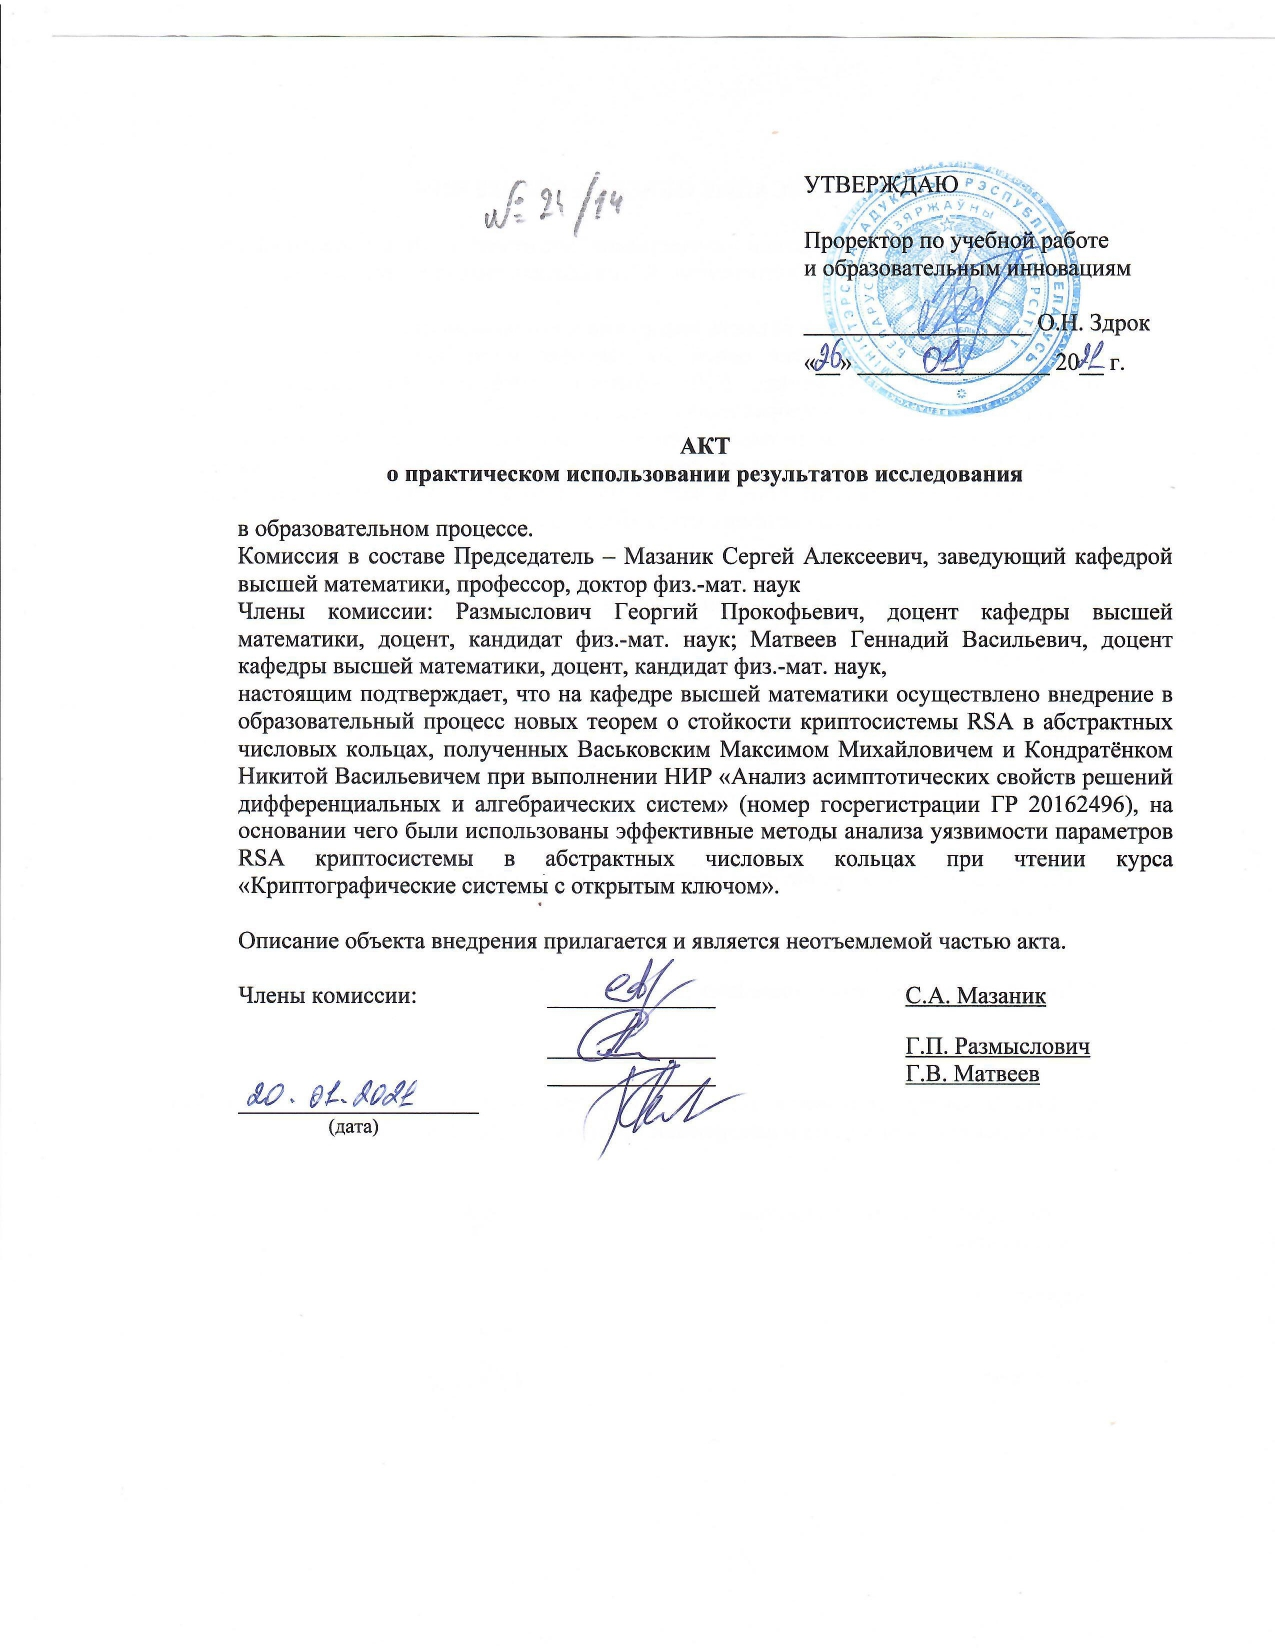
\includegraphics[width=0.85\textwidth]{../additional/Act_KondratyonokNV_page-0001.jpg}
\end{figure}

\begin{figure}[ht!]
    \centering
    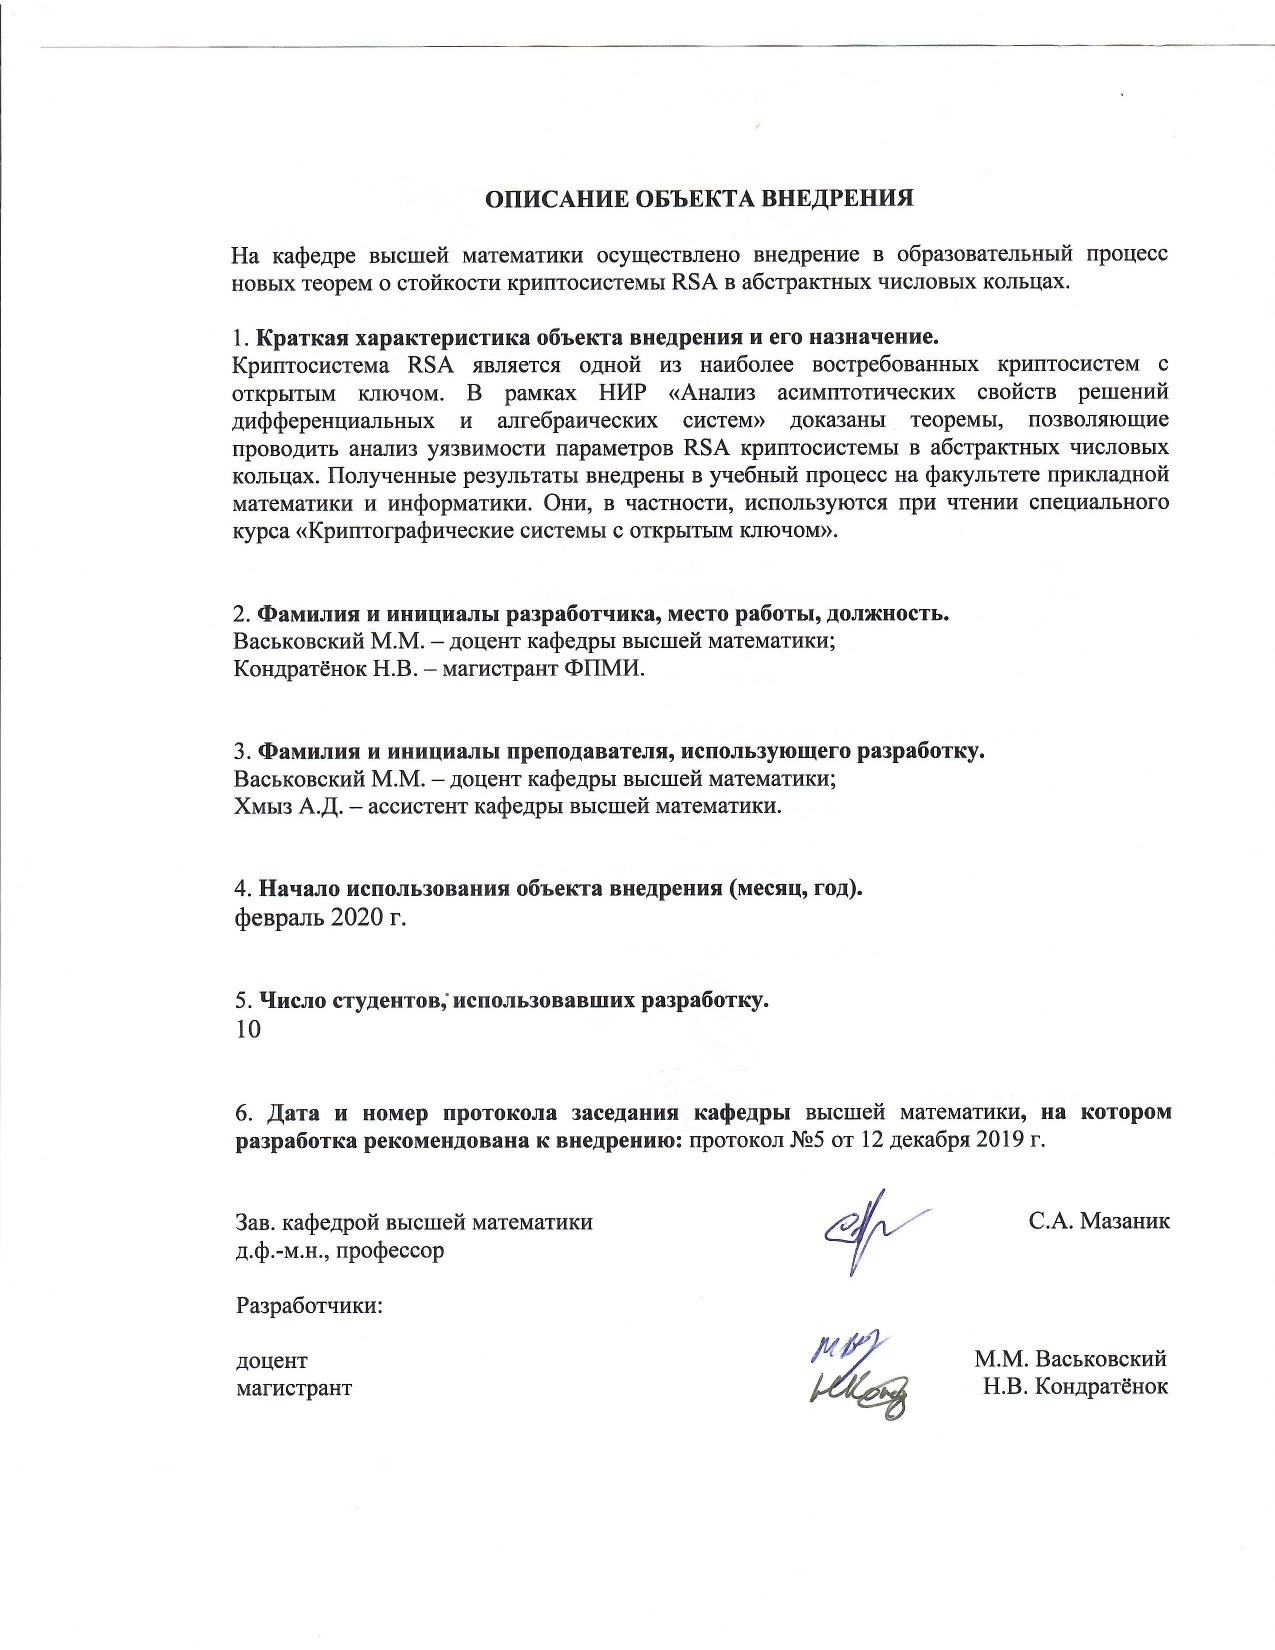
\includegraphics[width=0.85\textwidth]{../additional/Act_KondratyonokNV_page-0002.jpg}
\end{figure}

\refstepcounter{chapter}
\chapter*{\hfill ПРИЛОЖЕНИЕ~Б}
\addcontentsline{toc}{chapter}{ПРИЛОЖЕНИЕ Б Исходный код программы нахождения контрпримеров к теореме Кронекера-Валена}
\section*{Исходный код программы нахождения контрпримеров к теореме Кронекера-Валена}\label{section:Appendix_code}

\lstinputlisting{../additional/Find_Counterexample.r}

\onlyinsubfile{
    \subfile{_10_bibliography}
}

\end{document}
